\documentclass[11pt]{article}
\usepackage{acl}
\usepackage{times}
\usepackage{latexsym}
\usepackage{amsmath}
\usepackage{booktabs}
\usepackage{graphicx}
\usepackage{microtype}
\usepackage[T1]{fontenc}
\usepackage[utf8]{inputenc}
\usepackage{multirow}
\usepackage{url}
\graphicspath{{../results/figures/}}

\title{Cross-Lingual Hallucination Drift in LLMs:\\Does It Depend on Task Type?}

\author{
  Bhoomika Monthy Rajashekar \quad Devinn Chi \quad Chun Hsu \quad Anagha P Krishna \\
  Boston University \\
  \texttt{\{bhoomi02, dhchi, rexhsu, anaghapk\}@bu.edu} \\
  Advisor: Aaron Mueller
}

\begin{document}
\maketitle

%% ─── ABSTRACT ────────────────────────────────────────────────────────────────
\begin{abstract}
Large Language Models (LLMs) are known to hallucinate in non-English languages,
but whether this \textit{cross-lingual hallucination drift} is task-dependent
remains an open question. We evaluate \textbf{Aya Expanse 8B} across English,
Spanish, Italian, and Swahili on two structurally different tasks: factual
QA (TruthfulQA) and commonsense reasoning (XCOPA), using GPT-4o-mini as an
LLM-as-a-Judge evaluator. Italian is included in both benchmarks as a
confound-control language, enabling a within-language test that isolates task
type from language identity.

Our main finding is that drift is strongly task-dependent. TruthfulQA drift is
negligible for Spanish ($\Delta$HR\,=\,$-2.66$\,pp, $p=0.60$) and Italian
($\Delta$HR\,=\,$+1.34$\,pp, $p=0.80$). XCOPA Italian drift is similarly small
($+1.33$\,pp, $p=0.68$), while XCOPA Swahili drift is catastrophic
($+90.67$\,pp, $p<0.001$). The pairwise drift interaction score
$\Phi=-93.33$\,pp (Spanish/TruthfulQA vs.\ Swahili/XCOPA) is highly significant
($\chi^2=45.44$, $p<0.001$). A within-Italian test (fixing language and
varying only task) confirms task-dependency without any language-identity
confound ($\chi^2=16.98$, $p<0.001$).

Qualitative error analysis shows that Swahili XCOPA hallucinations are
predominantly \textit{incoherent} (27\% of failures, avg.\ 185 tokens),
unlike other cells which produce short wrong answers. Dual-judge validation
(GPT-4o-mini vs.\ Claude claude-sonnet-4-5 vs.\ human annotators on 50 Italian samples)
yields $\kappa=0.662$ for TruthfulQA/Italian but near-chance agreement
($\kappa=0.065$) for XCOPA/Italian, revealing inherent difficulty in judging
commonsense outputs. We also release an interactive Streamlit dashboard for
exploring all results.
\end{abstract}

%% ─── 1. INTRODUCTION ─────────────────────────────────────────────────────────
\section{Introduction}

Hallucination, defined as generating content that is factually incorrect or
unfaithful, is a well-documented failure mode of large language models
\cite{alansari2025survey}. As LLMs are deployed globally, a natural concern is
whether hallucination rates are systematically higher in non-English languages,
particularly low-resource ones with sparse training data
\cite{blasi-etal-2022-systematic}. This phenomenon is called
\textit{cross-lingual hallucination drift}: the change in hallucination rate
when a model operates in a non-English language.

A key recent study by \citet{ulislam-etal-2025-hallucinate} measured
token-level hallucination across 30 languages and 6 LLM families, finding that
length-normalized hallucination rates are \emph{uncorrelated} with language
resource level. This surprising result, however, was established on a single
task type: open-domain, knowledge-intensive long-form QA. Whether it holds for
structurally different tasks is unexplored.

Factual recall (TruthfulQA) and commonsense reasoning (XCOPA) make different
demands on the model. TruthfulQA requires retrieving stored parametric
knowledge; XCOPA requires selecting a culturally plausible cause or effect from
world knowledge anchored in the target language. These tasks may expose
fundamentally different multilingual failure modes.

We formally define the \textbf{Drift Interaction Score}:
\[
\Phi_l = \Delta\mathrm{HR}_{l,\,\text{TruthfulQA}}
       - \Delta\mathrm{HR}_{l,\,\text{XCOPA}}
\]
where $\Delta\mathrm{HR}_{l,t} = \mathrm{HR}_{l,t} - \mathrm{HR}_{\mathrm{en},t}$.
A large $|\Phi_l|$ indicates task-dependent drift for language $l$.

\paragraph{Contributions.}
\begin{itemize}
  \item We run a six-cell evaluation (en/es/it on TruthfulQA; en/it/sw on XCOPA)
        where Italian serves as a shared language enabling a confound-controlled
        within-language test.
  \item We confirm task-dependent drift via both a cross-task test
        ($\chi^2=45.44$, $p<0.001$) and a clean within-Italian test
        ($\chi^2=16.98$, $p<0.001$).
  \item We provide qualitative error analysis, an XCOPA causal-direction
        breakdown, and dual-judge reliability validation with manual inspection.
  \item We release an interactive Streamlit dashboard for result exploration.
\end{itemize}

%% ─── 2. RELATED WORK ─────────────────────────────────────────────────────────
\section{Related Work}

\paragraph{Cross-lingual hallucination.}
\citet{ulislam-etal-2025-hallucinate} is our most direct point of comparison.
They find no correlation between language resource level and hallucination in
long-form QA, using LaBSE-based semantic similarity as the evaluation signal.
Our work tests whether this null result generalizes across task types.
\citet{guerreiro-etal-2023-hallucinations} study hallucination in neural machine
translation, observing incoherence patterns in low-resource language pairs that
foreshadow our Swahili XCOPA findings.

\paragraph{Multilingual benchmarks.}
TruthfulQA \cite{lin-etal-2022-truthfulqa} provides adversarial factual
questions designed to elicit false beliefs held by humans.
\citet{qin-etal-2024-multilingual} survey multilingual LLM capabilities and
identify commonsense reasoning as a task type particularly sensitive to
language-specific cultural grounding.

\paragraph{LLM-as-a-Judge.}
Evaluating generation with a strong LLM judge is now standard practice for
open-ended tasks \cite{kang-etal-2024-comparing}. We follow this methodology
and add a dual-judge reliability check with human annotation to validate our
primary GPT-4o-mini judge.

\paragraph{Hallucination evaluation.}
\citet{li-etal-2023-halueval} introduce HaluEval, a hallucination benchmark for
knowledge-grounded tasks, noting that hallucination types vary substantially
across task categories, consistent with our error analysis finding that
incoherence dominates in Swahili XCOPA while wrong-answer errors dominate
in TruthfulQA.

%% ─── 3. METHODS ──────────────────────────────────────────────────────────────
\section{Methods}

\subsection{Datasets}

\paragraph{TruthfulQA \cite{lin-etal-2022-truthfulqa}.}
817 questions across 38 domains designed to elicit confident false beliefs. We
use the English original and Spanish and Italian translations from the
\texttt{alexandrainst/m\_truthfulqa} HuggingFace dataset.

\paragraph{XCOPA \cite{ponti-etal-2020-xcopa}.}
A cross-lingual commonsense causal reasoning benchmark spanning 11 languages.
Each example presents a premise and two candidate causes or effects; the model
selects the more plausible one. We use the English (SuperGLUE COPA), Italian,
and Swahili splits. Spanish is not available in XCOPA.

\paragraph{Italian as confound control.}
A key methodological choice is to include Italian in \emph{both} benchmarks.
This enables a within-language test: fixing language to Italian and varying
task, any significant difference in hallucination pattern must be attributable
to task type, not language identity or resource level. This directly addresses
the confound noted by our midway reviewer.

\paragraph{Sampling.}
We sample 150 examples per cell with random seed 42, yielding 900 total
evaluation instances across six cells.

\subsection{Target Model}

We evaluate \textbf{Aya Expanse 8B} (CohereLabs), a multilingual
instruction-tuned model explicitly trained for high-resource and low-resource
languages. We run 4-bit NF4 quantization (BitsAndBytes, double quant,
\texttt{float16} compute dtype) with greedy decoding and a maximum of 200 new
tokens. Prompts are zero-shot and written in the target language: TruthfulQA
uses a free-form answer format and XCOPA uses a forced-choice (A/B) format.
Inference runs on a Google Colab T4 GPU (15.8\,GB VRAM), with an estimated
total runtime of approximately 1.5--2\,hours for all six cells.

\subsection{LLM-as-a-Judge}

\paragraph{Primary judge.}
\textbf{GPT-4o-mini} receives each (question, model response) pair and labels
it \textit{Hallucinated} or \textit{Faithful} with a brief natural-language
justification \cite{kang-etal-2024-comparing}. GPT-4o-mini was chosen for its
strong multilingual comprehension across all four languages. Any response
receiving an \texttt{ERROR} label is automatically retried; all 900 items
received valid labels after retry.

\paragraph{Dual judge and manual validation.}
To validate judge reliability on Italian, a language the team can read
directly, we run a second judge pass using \textbf{Claude claude-sonnet-4-5} on a
stratified 50-sample subset per Italian cell. The same 50 samples are then
manually inspected to produce ground-truth human labels, following the
reviewer's suggestion to combine LLM dual-judging with manual inspection
\cite{kang-etal-2024-comparing}. This yields three-way inter-rater agreement
(GPT-4o-mini, Claude, human).

\subsection{Evaluation Metrics}

We compute the \textbf{hallucination rate}:
\[
\mathrm{HR}_{l,t} = \frac{\#\,\text{Hallucinated}}{N_{l,t}} \times 100\,(\%)
\]
where $N_{l,t}=150$ for all cells. Drift from English is
$\Delta\mathrm{HR}_{l,t} = \mathrm{HR}_{l,t} - \mathrm{HR}_{\mathrm{en},t}$.
Cohen's $\kappa$ is used for inter-rater agreement.
All code and outputs are publicly available on GitHub.\footnote{\url{https://github.com/bhoomi02-ai/Cross-Lingual-Hallucination-Drift-in-LLMs}}

\subsection{Statistical Tests}

\begin{itemize}
  \item \textbf{Mann-Whitney U}: tests whether per-item hallucination rates
        differ between English and each non-English language within a task.
  \item \textbf{Chi-squared ($2\times2$)}: (a) aggregate cross-task test on all
        non-English responses pooled; (b) within-Italian test on Italian-only
        responses.
  \item \textbf{Fisher's exact}: robustness check on the same tables.
\end{itemize}

\subsection{Error Categorization}

We categorize GPT-4o-mini judge justifications using keyword heuristics on the
reason text into five types: \textit{incoherent} (rambling, off-topic, or
structurally garbled), \textit{code-switching} (mid-response language switch),
\textit{fabricated} (hallucinated entities or facts), \textit{wrong answer}
(plausible but incorrect), and \textit{other}.

\subsection{Streamlit Dashboard}

We built an interactive dashboard using Streamlit for result exploration,
accessible by running \texttt{streamlit run app.py}. The dashboard has five
pages: (1) a KPI summary with $\Phi$ scores and the full six-cell HR table;
(2) interactive charts including HR bars, drift comparison, and a heatmap;
(3) a ``New Analyses'' page with tabs for XCOPA cause/effect breakdown,
dual-judge $\kappa$ visualization, and error category charts; (4) an example browser
for browsing individual model responses filtered by task, language, and label;
and (5) a reason analysis page with hallucination category distributions.

%% ─── 4. RESULTS ──────────────────────────────────────────────────────────────
\section{Results}

\subsection{Hallucination Rates and Drift}

Table~\ref{tab:hr} shows hallucination rates across all six cells. TruthfulQA
rates are similar across English (27.33\%), Spanish (24.67\%), and Italian
(28.67\%), with small and statistically non-significant drifts. XCOPA shows the
same near-English behavior for Italian (9.33\%, $+1.33$\,pp) but catastrophic
collapse for Swahili (98.67\%, $+90.67$\,pp).

\begin{table}[t]
\centering
\small
\begin{tabular}{llrrr}
\toprule
\textbf{Task} & \textbf{Lang} & \textbf{HR (\%)} & \textbf{$\Delta$HR} & \textbf{Avg Tok} \\
\midrule
TruthfulQA & en & 27.33 & ---         &  81.7 \\
TruthfulQA & es & 24.67 & $-2.66$\,pp & 108.0 \\
TruthfulQA & it & 28.67 & $+1.34$\,pp &  93.8 \\
\midrule
XCOPA      & en &  8.00 & ---         &  89.2 \\
XCOPA      & it &  9.33 & $+1.33$\,pp & 117.4 \\
XCOPA      & sw & 98.67 & $+90.67$\,pp & 185.0 \\
\bottomrule
\end{tabular}
\caption{Hallucination rate, drift from English, and average response token
count. $N=150$ per cell. Avg Tok = average tokens per response (all labels).}
\label{tab:hr}
\end{table}

\subsection{Task-Dependent Drift}

Table~\ref{tab:stats} presents all statistical tests.

\paragraph{Cross-task aggregate.}
Pooling all non-English responses, the hallucination outcome is not independent
of task type ($\chi^2=45.44$, $p<0.001$). The pairwise drift interaction score
$\Phi=-93.33$\,pp (Spanish/TruthfulQA vs.\ Swahili/XCOPA) far exceeds our
pre-specified minimum effect threshold of $|\Phi|\geq 2$\,pp.

\paragraph{Within-Italian confound test.}
Restricting to Italian only, task type strongly predicts hallucination outcome
($\chi^2=16.98$, $p<0.001$, Fisher OR\,=\,0.26, $p<0.001$). TruthfulQA/Italian
(HR\,=\,28.67\%) and XCOPA/Italian (HR\,=\,9.33\%) have very different absolute
rates even though both drift from English by only $\approx 1.3$\,pp. This test
eliminates the language-identity confound entirely: the same language produces
starkly different hallucination profiles across task types.

\begin{table*}[t]
\centering
\small
\begin{tabular}{p{3.2cm}p{4.8cm}rrl}
\toprule
\textbf{Test} & \textbf{Comparison} & \textbf{Stat.} & \textbf{$p$} & \textbf{Sig.} \\
\midrule
Mann-Whitney U & TruthfulQA: en vs es    & 11550.0 & 0.600    & No  \\
Mann-Whitney U & TruthfulQA: en vs it    & 11100.0 & 0.798    & No  \\
Mann-Whitney U & XCOPA: en vs it         & 11100.0 & 0.683    & No  \\
Mann-Whitney U & XCOPA: en vs sw         &  1050.0 & $<$0.001 & Yes \\
\midrule
Chi-squared (all non-EN)  & Aggregate ($\Phi = -46.67$\,pp) & 45.44 & $<$0.001 & Yes \\
Fisher exact (robustness) & Aggregate                       &  3.23 & $<$0.001 & Yes \\
\midrule
Chi-squared $|$ lang\,=\,it & it/TruthfulQA vs it/XCOPA & 16.98 & $<$0.001 & Yes \\
Fisher exact $|$ lang\,=\,it & it/TruthfulQA vs it/XCOPA &  0.26 & $<$0.001 & Yes \\
\bottomrule
\end{tabular}
\caption{Statistical test results. The bottom block restricts to Italian only, controlling for language identity.}
\label{tab:stats}
\end{table*}

\subsection{Figures}

Figure~\ref{fig:hr} shows hallucination rates across all six cells.
Figure~\ref{fig:drift} shows $\Delta$HR per non-English cell, making the
task-type interaction visually clear: Spanish and Italian bars are near zero
for both tasks, while Swahili XCOPA towers above all others.

\begin{figure}[t]
  \centering
  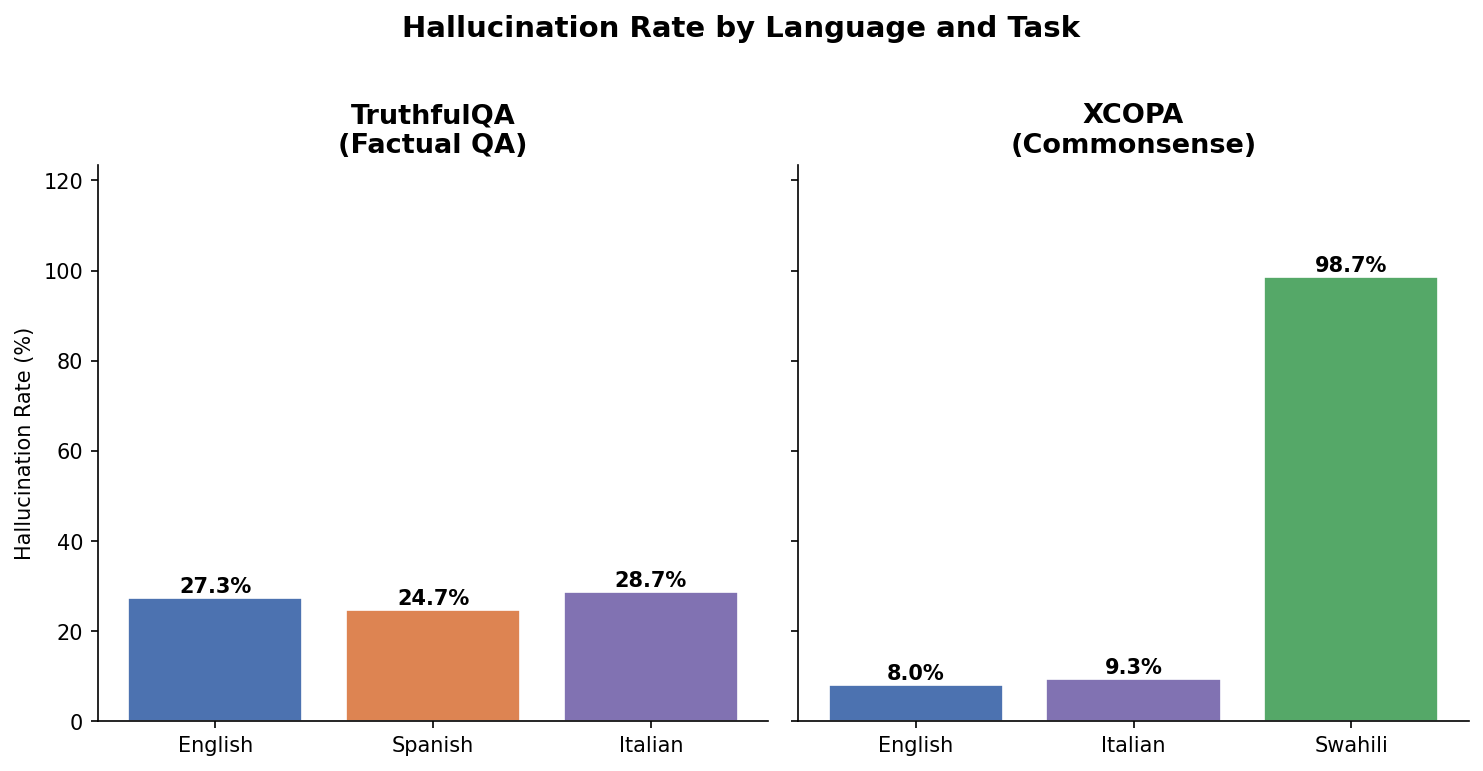
\includegraphics[width=\columnwidth]{hr_by_language_task.png}
  \caption{Hallucination rates by language and task. Italian behaves
  comparably to English in both tasks. Swahili XCOPA is near-total (98.67\%).}
  \label{fig:hr}
\end{figure}

\begin{figure}[t]
  \centering
  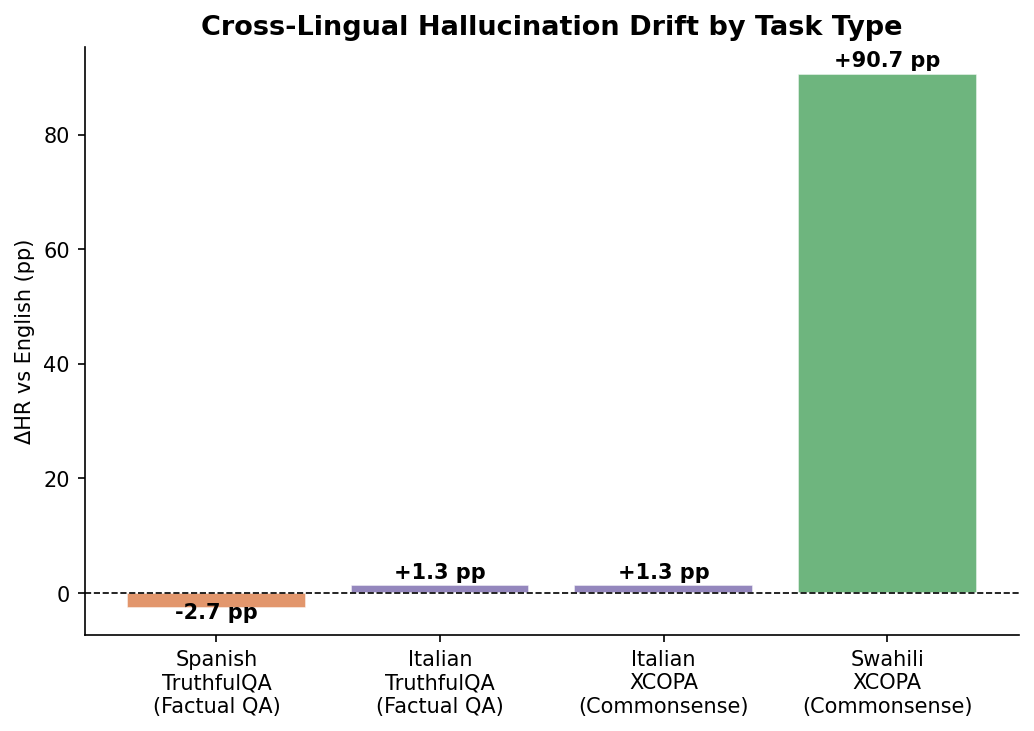
\includegraphics[width=\columnwidth]{drift_by_task.png}
  \caption{Cross-lingual drift ($\Delta$HR vs.\ English) per cell. Italian
  shows near-zero drift in both tasks; Swahili XCOPA shows catastrophic
  drift ($+90.67$\,pp).}
  \label{fig:drift}
\end{figure}

\subsection{Token Verbosity}

When hallucinating on XCOPA in Swahili, Aya generates an average of 185 tokens
per response, approximately twice the English XCOPA average (89 tokens) and
well above any TruthfulQA cell (82--108 tokens). This pattern is absent for
TruthfulQA in any language, where hallucinated and faithful token counts are
comparable. It suggests that Swahili XCOPA failures are not confident short
wrong answers but \textit{incoherent rambling}, corroborated by the error
analysis below.

\subsection{XCOPA Cause vs.\ Effect}

Table~\ref{tab:cause_effect} breaks XCOPA hallucination by question type.
For English and Italian, cause and effect rates differ by $\leq 1$\,pp and
neither difference is significant ($p=1.0$ and $p=0.27$ respectively).
Swahili shows near-total hallucination in both directions (cause: 96.43\%;
effect: 100.0\%), confirming that the Swahili collapse is not localized to
one causal direction but reflects a global failure on this language--task pairing.

\begin{table}[t]
\centering
\small
\begin{tabular}{llrrr}
\toprule
\textbf{Lang} & \textbf{Type} & \textbf{$N$} & \textbf{HR (\%)} & \textbf{$p$} \\
\midrule
en & cause  & 72 & 11.11 & \multirow{2}{*}{---} \\
en & effect & 78 &  5.13 &      \\
\midrule
it & cause  & 73 &  9.59 & \multirow{2}{*}{1.00} \\
it & effect & 77 &  9.09 &      \\
\midrule
sw & cause  & 56 & 96.43 & \multirow{2}{*}{0.27} \\
sw & effect & 94 & 100.00&      \\
\bottomrule
\end{tabular}
\caption{XCOPA hallucination rates by question type. $p$ = Fisher's exact
test within language. No significant cause/effect difference in any language.}
\label{tab:cause_effect}
\end{table}

\subsection{Error Analysis}

Table~\ref{tab:errors} shows hallucination categories per cell. Across
TruthfulQA and XCOPA English and Italian, the dominant error type is
\textit{wrong answer} (the model gives a plausible but incorrect response).
Swahili XCOPA is a clear outlier: 40 of 148 hallucinations (27\%) are
\textit{incoherent}, consistent with the token verbosity finding. No cell
shows meaningful fabrication or code-switching.

\begin{table}[t]
\centering
\small
\begin{tabular}{llrrrr}
\toprule
\textbf{Task} & \textbf{Lang} & \textbf{Fab.} & \textbf{Incoh.} & \textbf{W.Ans} & \textbf{Total} \\
\midrule
TruthfulQA & en & 0 &  0 & 14 &  41 \\
TruthfulQA & es & 1 &  1 & 11 &  37 \\
TruthfulQA & it & 1 &  0 & 15 &  43 \\
\midrule
XCOPA      & en & 0 &  0 &  5 &  12 \\
XCOPA      & it & 0 &  0 &  6 &  14 \\
XCOPA      & sw & 0 & 40 &  5 & 148 \\
\bottomrule
\end{tabular}
\caption{Hallucination error categories. Fab.\ = fabricated; Incoh.\ =
incoherent; W.Ans = wrong answer. \textit{Other} omitted for space.
$N$ = total hallucinated items per cell.}
\label{tab:errors}
\end{table}

\subsection{Dual-Judge Agreement}

Table~\ref{tab:kappa} shows inter-rater agreement on 50 Italian samples per
cell. For TruthfulQA/Italian, agreement is moderate: GPT-4o-mini vs.\ Claude
$\kappa=0.662$, GPT-4o-mini vs.\ human $\kappa=0.597$, Claude vs.\ human
$\kappa=0.712$. For XCOPA/Italian, all pairwise $\kappa$ values are near
chance (GPT vs.\ Claude $\kappa=0.065$, Claude vs.\ human $\kappa=0.065$,
GPT vs.\ human $\kappa=0.256$).

The low $\kappa$ on XCOPA/Italian is interpretively important. Since
XCOPA/Italian has only 14 hallucinated responses out of 150 (9.33\%), most
labels are \textit{Faithful} and boundary cases are sparse. Two strong LLM
judges genuinely disagree on these edge cases, suggesting that judging
commonsense forced-choice outputs is harder than judging factual QA. This does
not threaten the main results: the high-hallucination Swahili cell that drives
our primary finding produces unambiguously incoherent output.

\begin{table}[t]
\centering
\small
\begin{tabular}{lrrrr}
\toprule
\textbf{Cell} & \textbf{$n$} & \textbf{$\kappa$ G/C} & \textbf{$\kappa$ G/H} & \textbf{$\kappa$ C/H} \\
\midrule
TruthfulQA/it & 50 & 0.662 & 0.597 & 0.712 \\
XCOPA/it      & 50 & 0.065 & 0.256 & 0.065 \\
\bottomrule
\end{tabular}
\caption{Cohen's $\kappa$ for GPT-4o-mini (G), Claude claude-sonnet-4-5 (C), and
human (H) on 50 Italian samples per cell. Raw agreement: TruthfulQA/it = 0.84;
XCOPA/it = 0.38.}
\label{tab:kappa}
\end{table}

%% ─── 5. DISCUSSION ───────────────────────────────────────────────────────────
\section{Discussion}

\paragraph{Task type dominates language resource level.}
Our results provide strong and consistent evidence that hallucination drift is
task-dependent. TruthfulQA shows near-zero drift for Spanish and Italian
(both mid-resource languages with substantial training data coverage), and we
expect the same would hold for other mid-resource languages. XCOPA, however,
shows catastrophic drift for Swahili even though Italian (also non-English)
behaves comparably to English. The decisive variable is task type, not language
resource level.

\paragraph{Why does XCOPA Swahili collapse?}
Commonsense causal reasoning in XCOPA requires selecting a culturally plausible
cause or effect from world knowledge anchored in the target language. When the
model cannot produce a coherent answer in Swahili, it cannot even fall back on
a short wrong answer; it produces verbose, incoherent output instead. This
contrasts with TruthfulQA hallucinations, which are typically confident but
wrong short answers. The failure mode suggests the model's Swahili XCOPA
competence lies below the threshold needed for coherent forced-choice output,
not merely below the threshold for accuracy.

\paragraph{The Italian confound test is the cleanest result.}
The within-Italian chi-squared ($\chi^2=16.98$, $p<0.001$) shows that task
type predicts hallucination outcome even when language is held constant.
Notably, $\Phi_{\text{it}}=+0.01$\,pp, meaning Italian drifts by approximately the
same amount from English in both tasks ($\approx +1.3$\,pp). The significance
of the within-Italian test does not come from differential drift but from the
fact that the two tasks have very different absolute hallucination rates
(28.67\% vs.\ 9.33\% for Italian). This is the purest demonstration that task
structure, not language, determines the magnitude of the hallucination problem.

\paragraph{Implications for prior work.}
\citet{ulislam-etal-2025-hallucinate} found no correlation between language
resource level and hallucination in long-form QA. Our TruthfulQA results agree.
But our XCOPA Swahili result challenges the generalization of that finding:
task type is a major confound. Studies measuring hallucination drift on a
single task type risk drawing language-level conclusions that are actually
task-specific. Future work should evaluate drift across multiple task types
before attributing cross-lingual differences to language properties.

\paragraph{Limitations.}
First, we evaluate a single model; results may differ for models with different
multilingual training coverage. Second, Spanish and Swahili do not co-occur in
the same benchmark, so the cross-task $\Phi$ comparison conflates language and task
to some degree. The within-Italian test mitigates but does not fully resolve
this, as Italian is a mid-resource language; a truly low-resource language
appearing in both benchmarks would be ideal. Third, our error categorization
uses keyword heuristics on English judge reasons, which may be less reliable
for non-English error descriptions.

%% ─── 6. CONCLUSION ───────────────────────────────────────────────────────────
\section{Conclusion}

We measured cross-lingual hallucination drift in Aya Expanse 8B across six
language--task cells covering factual QA (TruthfulQA) and commonsense reasoning
(XCOPA) in English, Spanish, Italian, and Swahili. Hallucination drift is
strongly task-dependent: factual QA shows negligible drift for all languages
tested, while commonsense reasoning shows catastrophic collapse for Swahili.
A within-Italian test (same language, both tasks) confirms this is a
property of task type. Error analysis shows Swahili XCOPA failures are
incoherent rather than plausibly wrong, and dual-judge validation reveals that
commonsense forced-choice outputs are harder to judge reliably than factual QA
responses. Our findings suggest that task type should be treated as a
first-class variable in future cross-lingual hallucination studies.

%% ─── AUTHOR CONTRIBUTIONS ────────────────────────────────────────────────────
\section*{Author Contributions}

\textbf{Bhoomika Monthy Rajashekar} (Data \& Infrastructure) handled dataset
download and sampling for all six language--task cells including Italian, set
up the HuggingFace pipeline and prompt templates, and managed the GitHub
repository and data branch.

\textbf{Chun Hsu} (Evaluation \& Metrics) designed the LLM-as-a-Judge prompt,
implemented the hallucination rate, $\Delta$HR, $\Phi$, and per-language
$\Phi_l$ metrics for the within-Italian confound test, and built the Streamlit
interactive dashboard.

\textbf{Devinn Chi} (Experiments) ran zero-shot inference with Aya Expanse 8B
across all six cells with 4-bit NF4 quantization, managed output logging and
the failed-response retry pipeline, and ran GPT-4o-mini judge calls including
Italian labels.

\textbf{Anagha P Krishna} (Analysis \& Writing) conducted all statistical
significance tests, performed dual-judge validation with Claude and manual
annotation of Italian samples, carried out error categorization and the XCOPA
cause vs.\ effect breakdown, and wrote the final report.

%% ─── REFERENCES ──────────────────────────────────────────────────────────────
\bibliographystyle{acl_natbib}
\bibliography{references}

\end{document}
